\documentclass[11pt,a4paper]{article}
\usepackage[T1]{fontenc}
\usepackage{lmodern}
\usepackage[margin=25mm]{geometry}
\usepackage{amsmath,amssymb,amsthm,mathtools}
\usepackage{graphicx,booktabs,array,tabularx}
\usepackage{microtype}
\usepackage{caption}
\usepackage[numbers,sort&compress]{natbib}
\usepackage{xurl}
\usepackage{xcolor}
\usepackage[colorlinks=true,linkcolor=blue!40!black,citecolor=blue!40!black,urlcolor=blue!40!black]{hyperref}
\hypersetup{pdftitle={Affine constructions and incidence bounds for Kobon triangles},pdfauthor={Alejandro Zarzuelo Urdiales}}
\newtheorem{theorem}{Theorem}[section]
\newtheorem{lemma}[theorem]{Lemma}
\newtheorem{proposition}[theorem]{Proposition}
\newtheorem{corollary}[theorem]{Corollary}
\theoremstyle{definition}
\newtheorem{definition}[theorem]{Definition}
\theoremstyle{remark}
\newtheorem{remark}[theorem]{Remark}
\newcommand{\K}{K}
\newcommand{\Ks}{K_{\mathrm s}}
\newcommand{\G}{G}
\newcommand{\B}{B}
\newcommand{\N}{\mathbb N}
\newcommand{\R}{\mathbb R}
\newcommand{\Z}{\mathbb Z}
\newcommand{\floor}[1]{\left\lfloor#1\right\rfloor}
\newcommand{\ceil}[1]{\left\lceil#1\right\rceil}
\newcommand{\lean}[1]{{\small\nolinkurl{#1}}}
\DeclareMathOperator{\sgn}{sgn}
\setlength{\emergencystretch}{2em}
\captionsetup{font=small,labelfont=bf}
\setcounter{topnumber}{3}
\renewcommand{\topfraction}{0.9}
\renewcommand{\textfraction}{0.08}
\renewcommand{\floatpagefraction}{0.75}
\graphicspath{{figures/}}
\title{Affine constructions and incidence bounds\\for Kobon triangles}
\author{Alejandro Zarzuelo Urdiales}
\date{1 October 2026}
\begin{document}
\maketitle
\begin{abstract}
We refine a classical construction of triangular cells in real line arrangements and prove its geometry and counting in Lean. For every $n\ge4$ there is a simple affine arrangement with at least $\lfloor n(n-3)/3\rfloor+1+(n\bmod2)$ bounded triangular cells. A phase correction and controlled projective changes of affine chart give the additional triangles. We also give a quantitative exterior-extension rule for both parities, identify a boundary-resource obstruction to indefinitely repeating full-gain exterior steps, and formalize a compatible-seed instance of the Bartholdi--Blanc--Loisel doubling construction. For even arrangements without parallel pairs, local fan geometry yields multiplicity-sensitive upper estimates, including a sharp bound in the class with at most two finite multiple points. Exact finite certificates supplement the general lower construction. We distinguish theorems checked end to end in Lean from manuscript geometry and incomplete recursive formalization, and separate the affine refinement from numerical-priority claims.
\end{abstract}
\section{Introduction and relation to previous work}

Let $\K(n)$ be the maximum number of bounded triangular cells formed by $n$ distinct straight lines in $\R^2$. Multiple intersections and parallel pairs are allowed. Write $\Ks(n)$ for the maximum over \emph{simple} arrangements: no parallel pair and no three concurrent lines. Thus $\K(n)\ge\Ks(n)$. A triangular cell is a component of the complement of the lines whose closure is a nondegenerate triangle; arbitrary intersecting triples are not counted.

F\"uredi and Pal\'asti's trigonometric arrangements give the classical affine lower formula
\[
 \B(n)=\ceil{\frac{n(n-3)}3}\quad(n\ge3).
\]
This ceiling form is stated explicitly by Erickson; see also Felsner--Kriegel~\cite{furedipalasti1984,erickson1999,felsnerkriegel1999}. Our principal completed construction refines its constant term.

\begin{theorem}[Uniform affine refinement]\label{j:main}
For every $n\in\N$, a simple real-line arrangement realizes at least $\G(n)$ triangular cells, where $\G(n)=0$ for $n<3$, $\G(3)=1$, and
\begin{equation}\label{j:G}
 \G(n)=\floor{\frac{n(n-3)}3}+1+(n\bmod2),\qquad n\ge4.
\end{equation}
Consequently $\K(n)\ge\Ks(n)\ge\G(n)$. For $n\ge4$, in residue classes $0,1,\ldots,5$ modulo six, the gains $\G-\B$ are $1,1,0,2,0,1$.
\end{theorem}

The proof in Section~\ref{j:construction} constructs real lines and nonoverlapping triangular interiors. Its general Lean theorem uses only the standard logical axioms, not finite sampling or an assumed extension principle. The improvement is bounded by two; the leading terms $n^2/3-n$ are unchanged. The original F\"uredi--Pal\'asti projective counts already contain related constants. Our contribution is an explicit bounded-affine refinement and its geometric formalization; first numerical priority for the formula is not established by the source audit.

Several special families are stronger. Forge and Ram\'irez Alfons\'in construct a projective family whose affine deletion gives optimal orders $2\cdot2^t+1$~\cite{forge1998}. Bartholdi, Blanc and Loisel (BBL) give compatible doubling, with straight-line optimal families at $6\cdot2^t+1$ and $14\cdot2^t+1$~\cite{bbl2008}. Parpalak--Utkin establish the straight-line family $18\cdot2^t+1$~\cite{parpalakutkin2026}; its $108\cdot4^t-1$ triangles exceed $\G$ there by $6\cdot2^t-2$. A maximum with these families, extended by harmless distant lines, is another all-order lower bound. We therefore do not identify validity for all $n$ with pointwise numerical optimality.

For comparison, put $U_{\mathrm T}(n)=\floor{n(n-2)/3}$. The classical upper envelope and its residue refinements are reported by Cl\'ement--Bader~\cite{clementbader2007}. Blanc's stronger even-order estimate
\begin{equation}\label{j:blanc}
 \Ks(n)\le\floor{\frac{n(n-5/2)}3},\qquad n\ \text{even},
\end{equation}
requires simplicity~\cite{blanc2011}. In particular, nonsimple $14$-line examples with $54$ cells exceed the simple bound $53$. Section~\ref{jup:section} retains multiple points explicitly rather than assuming that smoothing preserves the count.

The remaining contributions are a quantitative boundary-defect extension, an obstruction to repeated full exterior gains, compatible real seed certificates and a geometric one-step BBL theorem, and local-to-global incidence estimates under explicit restrictions. These are stated with their mathematical and formal scopes. They replace the unrestricted successor claim proposed in the author's March manuscript~\cite{zarzuelo2026}, which remains unproved here. Recent coordinate and SAT-based work supplies comparison inputs, not uncredited discoveries~\cite{savchuk2025,maiorana2026,parpalakutkinGallery2026}. The complete research account, source audit, finite catalog and historical record remain available separately~\cite{zarzueloFull2026}.

\section{The uniform affine construction}\label{j:construction}

\subsection{Certificates for actual triangular cells}

Write a line $\ell$ as $a_\ell x+b_\ell y=c_\ell$, with affine evaluation $f_\ell$. For two nonparallel lines define
\[
 D_{\ell m}=a_\ell b_m-b_\ell a_m,\quad
 (X_{\ell m},Y_{\ell m})=(c_\ell b_m-b_\ell c_m,\ a_\ell c_m-c_\ell a_m),
\]
so that $p_{\ell m}=(X_{\ell m},Y_{\ell m})/D_{\ell m}$. Set
\[
 E(r;\ell,m)=a_rX_{\ell m}+b_rY_{\ell m}-c_rD_{\ell m},\qquad
 O(r;\ell,m)=E(r;\ell,m)D_{\ell m}.
\]
Then $O(r;\ell,m)=f_r(p_{\ell m})D_{\ell m}^2$ has the sign of the actual affine evaluation.

An increasing triple $i<j<k$ of pairwise nonparallel supports is \emph{certified} when its supports are nonconcurrent and, for every arrangement line $r$, the three values $O(r;i,j)$, $O(r;i,k)$, $O(r;j,k)$ have a common weak sign. This polynomial criterion permits other lines through vertices but excludes cuts through the interior.

\begin{lemma}\label{j:cell}
A certified triple determines a bounded triangular cell. Different increasing certified triples have disjoint interiors.
\end{lemma}
\begin{proof}
The three vertices are noncollinear. Each test line has one weak sign on their convex hull, and a strict sign on its interior: vanishing at an interior convex combination would force vanishing at all three vertices. The interior therefore lies in one strict sign cell of the arrangement. Conversely, the three supporting inequalities force positive barycentric coordinates, so that sign cell is exactly the triangle interior. It is convex and hence a component of the complement. If two certified interiors meet, their sign cells coincide; their three open sides then determine the same supports and the increasing triples agree.
\end{proof}

Lean proves nonemptiness, equality with the strict sign cell, and disjointness. The connected-component interpretation is the elementary argument above. Clearing rational denominators reduces finite certification to integer polynomial tests.

\subsection{Phase and repeated-index correction}

Use the classical trigonometric family
\begin{equation}\label{j:trig}
 \ell(\theta):\quad \sin\theta\,x+\cos\theta\,y=\sin(3\theta).
\end{equation}
Expansion gives $D(\ell(u),\ell(v))=\sin(u-v)$ and
\begin{equation}\label{j:sign}
 O(\ell(w);\ell(u),\ell(v))
 =4\sin^2(u-v)\sin(w-v)\sin(w-u)\sin(u+v+w).
\end{equation}
For $\theta_i=(i+a)\pi/n$, $0\le i<n$, consider the following selected triples:
\begin{equation}\label{j:residues}
 \begin{array}{c|c}
 a & i+j+k\pmod n\\ \hline
 1/2 & n-1,\ n-2\\
 1/6 & 0,\ n-1 .
 \end{array}
\end{equation}

Both arrangements are simple: the angles are distinct modulo $\pi$, and every three-angle sum is a half-integer multiple of $\pi/n$, never a multiple of $\pi$. For a selected triple, write
$\theta_i+\theta_j+\theta_k=q\pi+\varepsilon\pi/n$ with $\varepsilon=\pm1/2$. At a test index $r$ outside its supports, the sign of the last factor in~\eqref{j:sign}, evaluated at the pair $i,j$, is
$(-1)^q\sgn(r-k)$, because $|r-k+\varepsilon|<n$. The complete sign is therefore
\[
 (-1)^q\sgn(r-i)\sgn(r-j)\sgn(r-k),
\]
independent of the chosen pair. At a supporting index two evaluations vanish and the third causes no sign conflict. Lemma~\ref{j:cell} proves the selected cells.

For any residue $b$, the equation $i+j+k=b$ in $\Z/n\Z$ has $n^2$ ordered solutions. Each equality $i=j$, $i=k$, or $j=k$ excludes at most $n$ solutions. Two distinct residues thus retain at least $2n^2-6n$ ordered triples with distinct indices. Division by six gives $\B(n)$ for the half-phase choice.

\begin{lemma}[Phase correction]\label{j:phase}
The phase $a=1/6$ gives at least $\floor{n(n-3)/3}+1$ triangular cells for every $n\ge3$.
\end{lemma}
\begin{proof}
In residue zero all three repeated-index sets contain $(0,0,0)$, so their union has size at most $3n-2$. For residue $n-1$ retain the bound $3n$. If $T$ is the selected count, then
$6T\ge2n^2-6n+2$, and hence
$T\ge\ceil{(n(n-3)+1)/3}=\floor{n(n-3)/3}+1$.
\end{proof}

\subsection{Recovering bounded cells by changing the chart}

For $h\ne0$, the projective coordinate change
\[
 (x,y)\longmapsto\left(\frac{x}{h-x},\frac{y}{h-x}\right)
\]
transforms $(a,b,c)$ into $\Phi_h(a,b,c)=(ha-c,hb,c)$. Direct substitution gives
\begin{align}
 D(\Phi_h\ell,\Phi_hm)&=h(h-x_{\ell m})D(\ell,m),\notag\\
 E(\Phi_hr;\Phi_h\ell,\Phi_hm)&=h^2E(r;\ell,m),\notag\\
 O(\Phi_hr;\Phi_h\ell,\Phi_hm)&=h^3(h-x_{\ell m})O(r;\ell,m).\label{j:covariance}
\end{align}
A cut $x=h$ avoiding all old vertices preserves simplicity. If $h>0$ and a triangle lies left of the cut, or $h<0$ and it lies right of it, all three sign multipliers are positive. At an exposed vertex on the other side, the multiplier reverses.

\begin{lemma}[Exposed caps]\label{j:caps}
For odd $n\ge3$, a chart of the half-phase arrangement has at least $\B(n)+1$ bounded cells. For $n=6k+3$, $k\ge1$, another chart has at least $\B(n)+2$.
\end{lemma}
\begin{proof}
The abscissa of the intersection of $\ell(u)$ and $\ell(v)$ is
\[
 X(u,v)=\cos(2u)+\cos(2v)+\cos(2u+2v).
\]
Put $c=\cos(\pi/n)$ and $c_n=1+2c$. On the half-phase grid, the pair $(0,n-1)$ is uniquely rightmost, at $c_n$: the first two cosine terms are at most $c$ and the last at most one, with simultaneous equality only at this pair. Choose $0<h<c_n$ above all other abscissae. No selected triple in~\eqref{j:residues} contains this pair. For $n=2m+1$, substitution in~\eqref{j:sign} shows that the triple $(0,m,2m)$ has opposite weak signs at its exposed vertex and its other vertices, for each test line. Equation~\eqref{j:covariance} corrects exactly that sign. All old selected triangles survive and this extra triple becomes a cell.

For $n=6k+3=3m$, $m=2k+1$, the pairs $(m-1,m)$ and $(2m-1,2m)$ are exactly the leftmost vertices, both at $-c_n/2$. Here is an explicit exposure check. Write $z=\cos(u+v)$, $w=\cos(u-v)$; then
\[
 X=2z^2+2zw-1.
\]
For a nonadjacent, nonwrapping pair, $|w|\le2c^2-1$, and completing the square gives $X\ge-1-w^2/2>-c-1/2$, since
\[
 2c-1-(2c^2-1)^2=2(1-c)(2c^3+2c^2-1)>0\quad(n\ge9).
\]
For adjacent indices $w=c$ and
$X+c+1/2=(2z+1)(z+c-1/2)$. On the discrete grid, the next value above $z=-1/2$ is $\cos(2\pi/3-2\pi/n)$; it exceeds $1/2-c$ by $c(1-c+\sqrt3\sin(\pi/n))>0$. Thus equality occurs only at $u+v=2\pi/3,4\pi/3$, giving the stated pairs. The wrapping pair is rightmost.

Choose $h<0$ between these two abscissae and all others. No old selected triangle uses either pair. The two extra triples
\[
 (2k,2k+1,5k+2),\qquad(k,4k+1,4k+2)
\]
have, by~\eqref{j:sign}, the opposite weak sign at the exposed pair from the sign at their other vertices. The multiplier in~\eqref{j:covariance} reverses precisely the exposed-vertex sign. These triples are distinct and absent from the old selected list, proving the two-cell gain.
\end{proof}

\begin{figure}[tb]
\centering
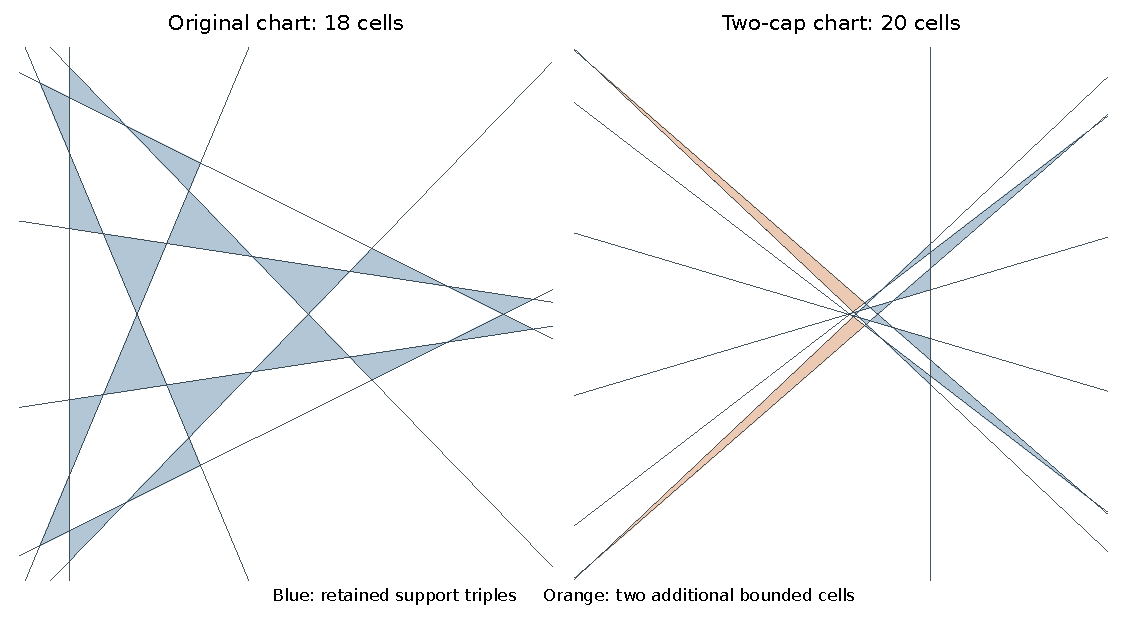
\includegraphics[width=.80\linewidth]{affine-chart.pdf}
\caption{Exact rational illustration of the two-cap chart at $n=9$: all 18 old cells survive and two become bounded. This realizes $\G(9)=20$, below the known optimum 21. Panels are independently rescaled; the general real-coordinate proof is symbolic.}\label{j:fig-chart}
\end{figure}

\begin{proof}[Proof of Theorem~\ref{j:main}]
For even $n\ge4$ use Lemma~\ref{j:phase}. For odd $n$ not divisible by three, $n(n-3)\equiv1\pmod3$, so $\B(n)+1=\floor{n(n-3)/3}+2$; apply the one-cap construction. For odd multiples of three at least nine, use the two-cap construction. Three nonconcurrent lines give the remaining nonzero small case. The same residue calculation gives the six stated gains.
\end{proof}

The exact deficit to the comparison polynomial is
\begin{equation}\label{j:gap}
 U_{\mathrm T}(n)-\G(n)
 =\floor{n/3}+\mathbf1_{n\equiv2\ (3)}-1-(n\bmod2),\qquad n\ge4.
\end{equation}
Thus the improvement is strict at infinitely many orders but leaves a linear gap. It constructs each order independently, not a nested chain from an arbitrary optimal seed.

\begin{figure}[tb]
\centering
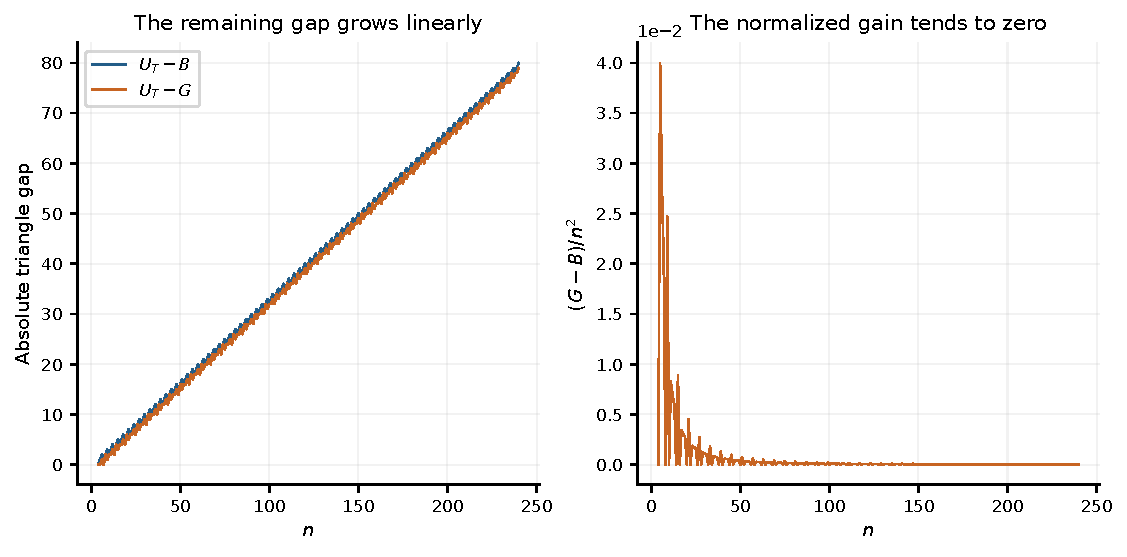
\includegraphics[width=.82\linewidth]{normalized-gap.pdf}
\caption{The exact deficit resolves the bounded gain over $\B$; normalized growth shows the unchanged leading coefficient. $U_{\mathrm T}$ is an external comparison polynomial, not a new unrestricted upper theorem.}\label{j:fig-gap}
\end{figure}

\section{Exterior extensions and their boundary resource}
\label{jext:section}

Exterior addition has precedents in BBL and Blanc~\cite{bbl2008,blanc2011}.
The contribution here is an explicit geometric certificate, a quantitative
defect formulation for both parities, and an obstruction to repeatedly
demanding the full gain proposed in March~\cite{zarzuelo2026}.

Let $A$ be a simple $n$-line arrangement, $n\ge3$, with equations $f_i=0$ and
vertices $p_{ij}$.  A linear functional $w$ is admissible if it is nonzero
on every line direction.  At $p_{ij}$ choose support directions $u_i,u_j$
with $w(u_i)=w(u_j)=1$.  Call the pair \emph{visible} if, for every old
line $f_k=0$, the numbers
\[
 f_k(p_{ij}),\quad Df_k(u_i),\quad Df_k(u_j)
\]
have one common weak sign.  This condition certifies an empty unbounded
wedge using only old data.

\begin{theorem}[Verified exterior realization]
\label{jext:visible}
If $A$ contains $T$ distinct certified triangles and $c$ distinct pairs
visible from an admissible $w$, adjoining $w(x)=H$, where
$H>\max_{i<j}w(p_{ij})$, gives a simple arrangement with at least $T+c$
triangles.
\end{theorem}
\begin{proof}
The new line is nonparallel to every support, misses all old vertices,
and lies beyond every old bounded cell.  Thus simplicity and old triangles
are preserved.  A visible pair has new vertices
$p_{ij}+(H-w(p_{ij}))u_i$ and $p_{ij}+(H-w(p_{ij}))u_j$.
Their affine evaluations are
$f_k(p_{ij})+(H-w(p_{ij}))Df_k(u)$, so all three vertices have one weak
sign against every old line.  The triangle is nondegenerate and empty.
Distinct pairs give distinct new support triples, all containing the
new line and hence distinct from the old triples.
\end{proof}
This is \lean{Exterior.extension}, a real-coordinate Lean theorem with
no parity restriction or assumed future count.

Write $T=t(A)$, $d=n(n-2)-3T$, and let $b$ count unbounded two-sided cells.
The quantity $d$ counts unused bounded elementary segments: a segment
in a simple arrangement supports at most one triangle.

\begin{proposition}[Boundary-defect extension]
\label{jext:defect}
For $n\ge3$, define
\begin{equation}
 g(n,T)=\ceil{\frac{n-1}{2n}\max\{3,\,3T-n(n-3)\}}.
 \label{jext:gain}
\end{equation}
Then $\Ks(n)\ge T$ implies $\Ks(n+1)\ge T+g(n,T)$.
\end{proposition}
\begin{proof}
There are $2n$ free rays, of which $2b$ belong to wedges.  At an unpaired
ray's endpoint $L\cap M$, both incident segments of $M$ are bounded.
They cannot both support triangles, since those triangles would share
the unique bounded segment of $L$ starting there.  Charge this ray to
an unused segment of $M$.  Each unused segment receives at most two
endpoint charges, giving $b+d\ge n$.  Convex-hull vertices of the finite
intersection set supply at least three wedges, so $b\ge\max\{3,n-d\}$.

The two rays of a wedge are consecutive in cyclic direction order.
Among the $2n$ admissible normal sectors, each wedge is visible in
exactly $n-1$: positivity selects $n$ consecutive oriented directions.
Thus some sector sees at least $\ceil{(n-1)b/(2n)}$ wedges.  Apply
Theorem~\ref{jext:visible}.  The expression is nondecreasing in $T$,
so a lower count can replace the witness's actual count.
\end{proof}
The cyclic count and defect arithmetic are formalized.  The universal
ray-charging and geometric cyclic-data extraction remain manuscript
proofs; the proposition is not claimed as an end-to-end Lean theorem.

If $n=2m+1$ and $d\le2$, then $b\ge2m-1$.  Averaging forces at least
$m$ visible wedges, since
$2m(2m-1)>(4m+2)(m-1)$; no sector can contain more than $m$ disjoint
ray pairs.  Hence every such odd input admits the full gain $m$.
For either parity the exact full-gain test is that some sector contains
$\floor{n/2}$ wedge pairs.  The defect rule itself can be iterated
without assuming this stronger condition persists.

Repeated exterior additions have a finite boundary resource.  If $b_r$
is the wedge count and $c_r$ the gain, each new triangle consumes an
old wedge.  No new free ray appears at an old vertex, and new wedges
can use only the two free rays of the added line.  Therefore
\begin{equation}
 b_{r+1}+c_r\le b_r+2,\qquad
 \sum_{j<r}c_j\le b_0+2r-3.
 \label{jext:budget}
\end{equation}
Quadratically accumulating full gains cannot continue indefinitely.
For the saved $49:767$ seed, $b_0=47$; gains $24$ and $25$ in two
exterior steps would leave at most two wedges, contradicting $b\ge3$.
This does not refute a recurrence for maxima using reconstruction.

\begin{figure}[tb]
\centering
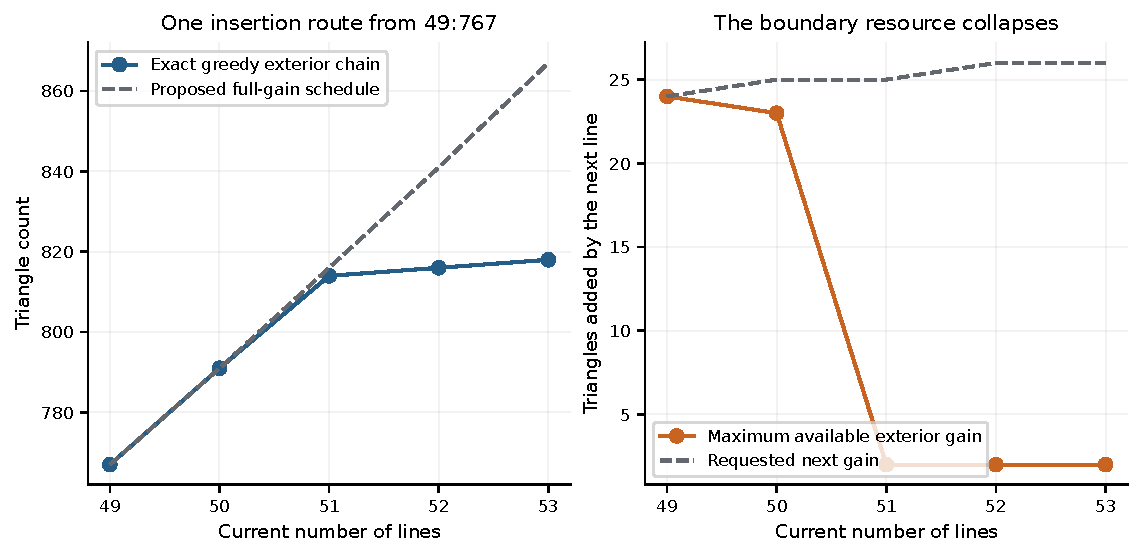
\includegraphics[width=.82\linewidth]{successor-49-resource.pdf}
\caption{One exact exterior chain from $49:767$. Its gains $24,23,2,2$ produce counts $791,814,816,818$. The displayed capacities belong to these particular arrangements; the general obstruction is the wedge budget~\eqref{jext:budget}, not an upper bound for $\K$.}\label{jext:figure}
\end{figure}

Conditionally, $F(n+1)\ge F(n)+\floor{n/2}$ yields
\[
 F(n)\ge F(s)+\floor{(n-1)^2/4}-\floor{(s-1)^2/4}.
\]
The recurrence remains unproved for $\K$.  Nevertheless its $49$-seed
numerical target is independently unconditional:
\begin{equation}
 \K(n)\ge\floor{(n-1)^2/4}+191\qquad(n\ge49).
 \label{jext:49}
\end{equation}
Lean proves this from the finite 49/50 witnesses and the classical
baseline for $n\ge51$; it does not construct a nested full-gain chain.

\section{Compatible seeds and geometric doubling}
\label{jfam:section}

The doubling mechanism is due to Bartholdi--Blanc--Loisel
(BBL)~\cite{bbl2008}.  Our completed formal result is one actual geometric
step, with explicit compatible input.

\begin{theorem}[Verified BBL step]
\label{jfam:doubling}
Let $q=4r\ge20$, $0<\varepsilon<\tan(\pi/(2q))$, and $t_j=\tan(j\pi/q)$.
Take $Y_0:y=0$ and $L_j:y=m_j(x-a_j)$ on the ordered grid
\[
 (a_j)=(-t_{q/2-1},\ldots,-t_1,-\varepsilon,
              \varepsilon,t_1,\ldots,t_{q/2-1}).
\]
Assume simplicity, all $q-1$ triangular cells with supports
$(Y_0,L_j,L_{j+1})$, positive height at
$L_{q/2-1}\cap L_{q/2}$, and $T$ distinct
certified triangles.  Then $\Ks(2q+1)\ge T+q^2$.
\end{theorem}
\begin{proof}[Proof mechanism]
Set $\beta_i=-\pi/2+(i+1/2)\pi/q$ and add
\[
 y=\kappa\bigl(\sin(2\beta_i)+\delta\cot\beta_i\bigr)
                  (x-\tan\beta_i),\qquad 0\le i<q.
\]
Exact intersection identities first give the required crossing order
for sufficiently small $\delta>0$, then for sufficiently small
$\kappa>0$.  Simplicity and the exceptional complementary crossings
are included in this proof.  The row count gives at least
$2\binom{q+1}{2}-q=q^2$ mixed triangles, each certified geometrically.
Old triangles off $Y_0$ persist; alternating cap signs replace the
noncentral triangles on $Y_0$, and the central triangle survives.
Their support types make the two lists disjoint.
\end{proof}
The complete statement is \proofref{Kobon/BBLDoubling.lean}{15}{\lean{BBLDoubling.doubling}}; neither crossing
order nor future triangle retention remains an external premise.

Our compatible eleven-line realization uses $Y_0$ and $x-v_jy=a_j$, with
\[
 (v_j)=\tfrac1{10}(15,-2,14,1,4,-4,5,-3,12,-5),
\]
and the same grid at $q=10$.  For every real
$0<\varepsilon\le10^{-5}$, Lean certifies simplicity, 32 triangles,
nine distinguished triangles, and five pairs visible from $w=(10,-13)$.
The count 32
is inherited from the Honma-based seed presented by
Savchuk~\cite{savchuk2025}; the contribution is the compatible realization
and uniform parameter proof.

For $q=10\cdot2^t$, the published BBL iteration applied to this seed gives
the paper-supported family
\begin{equation}
 T_q=\frac{q^2-4}{3},\qquad
 \Ks(q+1)\ge T_q,\qquad
 \Ks(q+2)\ge T_q+q/2-1.
 \label{jfam:families}
\end{equation}
The odd formula sums $T_{2q}=T_q+q^2$, preserving the certified segment
defect $q^2-1-3T_q=3$; the even formula uses
Proposition~\ref{jext:defect}.  A parameter may be chosen separately
for each finite depth.  These infinite statements are not yet
end-to-end Lean theorems.  The stronger even value $T_q+q/2$ requires
the additional recursive hypothesis of $q/2$ visible pairs; proved
visibility components and finite examples do not discharge that
invariant automatically.

Finite Lean checkpoints include
\[
 \begin{gathered}
 11:32,\quad12:37,\quad21:132,\quad22:142,\quad41:532,\quad42:552,\\
 81:2132,\quad82:2172,\quad161:8532,\quad162:8612.
 \end{gathered}
\]
The larger $321:34132$, $322:34292$, and $641:136532$ witnesses passed
two independent exact counters, but are outside the Lean catalogue.
The $642:136852$ candidate lacks its completed second count.
For the saved $81$- and $161$-line witnesses, exact projective face
censuses already equal the bounded-cell counts. A change of affine chart
alone therefore cannot improve those particular witnesses. This finite
obstruction does not apply to a different arrangement at the same order.

The true-grid 21-line parameter family is separately verified with
132 triangles and all 19 distinguished triangles.  Next-grid saturation
and the sorting permutation are also proved.  Recursive Lean iteration
still requires returning the full geometric witness, transporting its
duplicate-free triangle list, retaining the central triangle independently
of that list, and inducting on
$\exists\eta>0\ \forall\varepsilon\in(0,\eta)\ \exists$ a compatible seed.
The next central apex is exactly the old one.  This would certify the
$q=20\cdot2^t$ tail; even companions need a separate visibility invariant.

The verification pipeline also certifies a corrected five-line
normalization throughout $0<\varepsilon\le10^{-5}$, with five triangles,
three distinguished triangles and two visible pairs. For the
Parpalak--Utkin 19-line seed, a separate exact interval calculation
checks 107 triangles and 17 distinguished triangles on
$0<\varepsilon\le10^{-3}$; this is not a new infinite-family Lean theorem.
The dyadic optimal family retains Forge--Ram\'irez Alfons\'in attribution
\cite{forge1998}; the compatible 19-line reproduction and
$18\cdot2^t+1$ straight-line family retain Parpalak--Utkin attribution
\cite{parpalakutkin2026}.  Neither inherited methods nor newly archived
checkpoints are claimed as new numerical records.
For completeness, the known odd formulas at $q=4\cdot2^t$ and
$q=18\cdot2^t$ are $(q^2-1)/3$ and $q^2/3-1$, respectively.
Their odd defects are zero and two, so Section~\ref{jext:section}
gives the corresponding simple even companions by adding $q/2$.

\section{Multiplicity-sensitive upper estimates}
\label{jup:section}

Throughout this section $n\ge4$ is even and the $n$ distinct affine lines are pairwise nonparallel. These restrictions are essential: the conclusions concern arrangements in stated subclasses, not a new global upper bound for $\K$. The proofs below are ordinary geometric arguments; their formalization status is stated at the end.

Let $T$ count bounded triangular cells, and $t_r$ finite points incident to $r$ lines. The \emph{core} consists of the points with $r\ge3$; put
\[
 q=\sum_{r\ge3}t_r,\qquad I=\sum_{r\ge3}rt_r,\qquad
 S=\sum_{r\ge3}r(r-2)t_r,\qquad \delta=n(n-2)-3T.
\]
Let $h$ count lines meeting the core. A bounded elementary segment joins consecutive intersections on a line. Write $E$ for their total, $U$ for those incident to no triangle, and $D_1,D_2$ for shared sides with respectively one and two core endpoints. A shared side cannot have two ordinary endpoints: both adjacent triangles would then have the same three supporting lines. Pair counting and point-line incidence counting give
\begin{equation}
 E=\sum_{r\ge2}rt_r-n=n(n-2)-S,\qquad
 3T=E-U+D_1+D_2,\qquad
 \delta=S+U-D_1-D_2.
 \label{jup:identity}
\end{equation}

\begin{lemma}[Clean-line parity]
\label{jup:clean}
One has $n-h\le2U+D_1$, and consequently
\begin{equation}
 2\delta\ge n+2S-h-3D_1-2D_2.
 \label{jup:budget}
\end{equation}
\end{lemma}
\begin{proof}
Adapt Blanc's local parity argument~\cite{blanc2011}. A clean line $L$ avoids the core. Place it horizontally; label its crossings $1,\ldots,n-1$, with transverse lines $R_i$. Let $p_i^\pm$ be the faces above/below the interval between crossings $i,i+1$, and $r_i^\pm$ the transverse elementary pieces incident to crossing $i$. The exterior faces $p_0^\pm,p_{n-1}^\pm$ are unbounded. Intervals on $L$ are unshared.

Suppose every bounded $r_i^\pm$ belongs to exactly one triangle. If neither $p_1^\pm$ is triangular, both $r_1^\pm$ are unused; at least one is bounded since $R_1$ meets another transverse line. Thus, after reflection, $p_1^+$ is triangular and $p_1^-$ is not.

Inductively, $p_i^+$ is nontriangular for even $i$, and $p_i^-$ for odd $i$; moreover, if both $p_{i-1}^\pm$ are nontriangular, the other face at interval $i$ is triangular. For the even step, if $p_{i-1}^+$ is triangular, $p_i^+$ cannot be: they would share $r_i^+$. Otherwise both previous faces are nontriangular. This case requires $i\ge4$. The earlier even step makes $p_{i-2}^+$ nontriangular, so $r_{i-1}^+$ is unused and therefore unbounded. Hence $R_{i-1}\cap R_i$ lies below $L$, making $r_i^-$ bounded. Its left face is nontriangular, forcing $p_i^-$ triangular and $p_i^+$ nontriangular. The odd step exchanges signs.

Since $n-2$ is even, $p_{n-2}^+$ is nontriangular. If its lower neighbor is also nontriangular, both last transverse pieces are unused and one is bounded, a contradiction. Otherwise $r_1^-$ and $r_{n-1}^+$ are unused. The intersection $R_1\cap R_{n-1}$ lies below or above $L$, making the corresponding unused piece bounded, again a contradiction.

Each clean line therefore meets a bounded unused or shared transverse segment. Charge it to one such segment. An unused segment receives at most two charges, one per ordinary endpoint; a $D_1$ segment receives at most one, and a $D_2$ segment none. This proves the charging inequality; combine it with~\eqref{jup:identity}.
\end{proof}

The nonparallel hypothesis enters twice, through intersections of transverse lines. Three parallel verticals and one horizontal line would leave the horizontal line clean, but all its transverse pieces unbounded. Excluding only parallel-participating lines from the charging set therefore does not repair the argument.

\begin{lemma}[Fan bounds]
\label{jup:fan}
At an $r$-fold core point, $r\ge3$, let $d_1,d_2$ count incident shared segments with ordinary and core other endpoints. Then
\[
 d_1\le2r-3,\qquad 3d_1+d_2\le6r-6.
\]
If $d_2\le1$, then $d_1\le2r-4$.
\end{lemma}
\begin{proof}
Among the $2r$ cyclic rays, no $r-1$ consecutive rays can be counted by $d_1$. Their $r$ neighboring triangular sectors would have a common opposite supporting line: at each ordinary endpoint, the two adjacent opposite supports coincide. That line would meet $r+1$ consecutive rays, including an opposite pair, forcing it through the center and degenerating a triangle. Counting selected rays in all windows of length $r-1$ gives
\[
 (r-1)d_1\le2r(r-2)<(r-1)(2r-2).
\]
Together with $d_1+d_2\le2r$, this proves the first two bounds.

Suppose $d_2\le1$ and $d_1\ge2r-3$. Not all sectors can be triangular, since deleting at most one core-ended ray would leave a forbidden selected run. Two separated nontriangular sectors, or three consecutive ones, exclude at least four shared rays. Thus there are either one or two adjacent nontriangular sectors. One leaves a shared path of length $2r-2$; removing at most one $d_2$ ray leaves at most two selected runs, of total capacity $2(r-2)<2r-3$. Two adjacent sectors leave at most $2r-3$ shared rays, all necessarily selected in one forbidden run. Both possibilities contradict the run bound.
\end{proof}

\begin{theorem}[Restricted upper estimates]
\label{jup:upper}
Under this section's hypotheses,
\begin{equation}
 2\delta\ge n+\sum_{r\ge3}(2r^2-11r+6)t_r.
 \label{jup:weighted}
\end{equation}
If $q\le2$, then
\begin{equation}
 T\le\floor{\frac{n(n-5/2)}3}+1.
 \label{jup:two-core}
\end{equation}
The sharper defects for $q=0$ and $q=1$ are respectively $\delta\ge n/2$ and $\delta\ge n/2-1$.
\end{theorem}
\begin{proof}
Summing the fan bound gives $3D_1+2D_2\le6I-6q$. Since $h\le I$, equation~\eqref{jup:budget} proves~\eqref{jup:weighted}.

For $q\le2$, every core point has $d_2\le1$, so $D_1\le2I-4q$. Also $D_2\le1$ and $h\le I-D_2$: a core-to-core segment identifies a line counted twice in $I$. Therefore
\[
 2\delta\ge n+\sum_{r\ge3}(2r^2-11r+12)t_r-D_2
 \ge n-3q-D_2\ge n-7,
\]
using $2r^2-11r+12=-3+(r-3)(2r-5)\ge-3$. Parity gives $2\delta\ge n-6$, proving~\eqref{jup:two-core}. For $q=0,1$, one has $D_2=0$; the same inequality gives $2\delta\ge n$ and $2\delta\ge n-3$, respectively, with the latter rounding to $n-2$.
\end{proof}

If all core multiplicities are at least five, their weights in~\eqref{jup:weighted} are positive, since $2r^2-11r+6=1+(r-5)(2r-1)$; thus $T\le\floor{n(n-5/2)/3}$. Bound~\eqref{jup:two-core} is attained within its class at $n=8,14,26,50$ by attributed exact witnesses with $15,54,204,792$ triangles~\cite{maiorana2026,parpalakutkinGallery2026}; no unrestricted optimality or first numerical priority follows.

More generally, a nonnegative total weight suffices for the same simple-style polynomial. The weights at multiplicities three and four are $-9$ and $-6$, so the estimate does not control an arbitrary core of low-multiplicity points. Any stronger global argument must handle that deficit rather than omit the shared-side term.

Shared-edge accounting is indispensable. The six lines
\[
 x=0,\ y=0,\ x+y=3,\ x-y=0,\ 2x+y=3,\ x+2y=3
\]
give six triangular cells and six shared radial segments at $(1,1)$, with $d_1=d_2=3$. This disproves only a literal local incidence reading of Cl\'ement--Bader's shared-pair statement~\cite{clementbader2007}, not their final theorem.

\begin{figure}[tb]
\centering
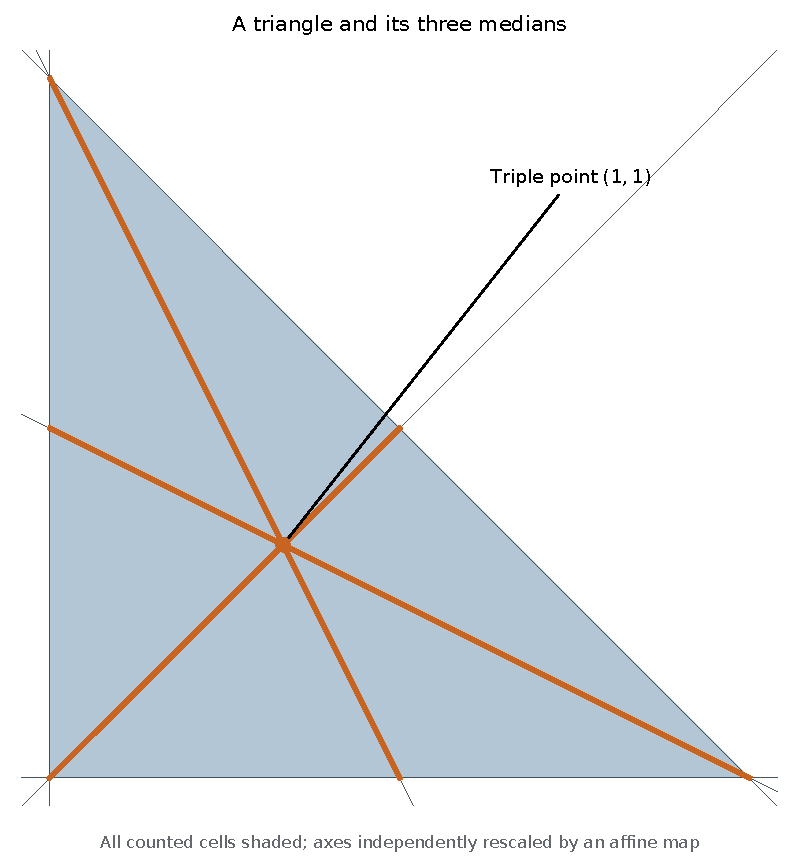
\includegraphics[width=.50\linewidth]{shared-fan.pdf}
\caption{Six exact triangular cells and six shared radial sides at the central triple point. Ordinary-ended and core-ended sides must be counted separately. The example and its uncut, pairwise disjoint interiors are proved in Lean.}\label{jup:figure}
\end{figure}

Smoothing is not automatically nondecreasing either. The four generic local resolutions of a retained Maiorana $14{:}54$ witness have exact counts $52,52,53,52$. Unchanged nonzero pair-direction and triple-determinant signs, together with the two resolved triple signs, exhaust sufficiently small simple perturbations. The finite counts are independently checked; this continuity-based classification is not a Lean theorem.

For gallery inputs of orders $8,14,20,26,32,38,50$, all 132 recorded local
resolutions were realized by exact private-line offsets. Their respective
best nearby simple counts are $14$, $51$, $114$, $203$, $313$, $448$, and $791$. Thus even a universal
loss-at-most-one rule fails for resolving these collinear cores.
These finite sign-stability obstructions concern the specified input types;
they do not bound all simple arrangements at those orders.

Lean verifies the shared-fan example, real fan obstruction and cyclic count. Global elementary-edge extraction, clean-line charging, and the sharper $d_2\le1$ refinement remain manuscript arguments; the Lean aggregate budget is conditional on their hypotheses. Parallel classes also require a separate argument.

\section{Finite consequences and verification}\label{j:verification}

Let $C(n)$ be the largest count among the saved exact certificates at order $n$, or zero if none is present. The finite-enhanced bound
\begin{equation}\label{j:envelope}
 \K(n)\ge L(n):=\max\{\G(n),C(n)\},\qquad n\in\N,
\end{equation}
is proved in Lean. The release contains 138 distinct coordinate identities, 104 simple; published inputs retain their attribution. For $n>195$, this saved envelope equals $\G(n)$. Neither catalog size nor~\eqref{j:envelope} asserts an exhaustive numerical optimum.

\begin{table}[tb]
\centering\small
\begin{tabular}{@{}llp{.35\linewidth}@{}}
\toprule
Order(s) $n$ & Certified counts, in order & Role\\
\midrule
$28,30,34$ & $238,275,357$ & Earlier attributed inequalities\\
$44$ & $608$ & Simple witness matching~\eqref{j:blanc}\\
$39,47,48$ & $470,691,721$ & One above earlier retained counts\\
$51,53,54,55$ & $818,885,919,955$ & One above earlier retained counts\\
$59,60,99,195$ & $1103,1141,3170,12482$ & One above earlier retained counts\\
\bottomrule
\end{tabular}
\caption{Selected simple certificates. Improvements are relative to the project's earlier witnesses, not asserted global records. The supplement contains every coordinate identity and the complete orders 3--60 table.}\label{j:finite}
\end{table}

The March-associated values at $28,30,34$ lines now have independent certificates despite the unfinished original extension argument~\cite{zarzuelo2026,oeisA006066}. They are not claimed as first numerical discoveries: $30:275$ appears in BBL, and $34:357$ follows from the older perfect 33-line construction and exterior addition~\cite{bbl2008,forge1998}. The exact $43:587\to44:608$ extension, together with Blanc's external upper theorem, gives $\Ks(44)=608$, not equality for $\K(44)$. The earlier proposed additional-line formula $q^2/3+q+1$ at $n=q+3$, $q=6\cdot2^t$, is uniformly superseded numerically by $\G(q+3)=q^2/3+q+2$.

The finite certificates apply Lemma~\ref{j:cell} to polynomial signs and distinct support triples. Two independent rational counters check their complete triangle sets. This also reproduces all fifteen Maiorana $14:54$ inputs and ten gallery witnesses from Parpalak--Utkin, including $26:204$ and $50:792$~\cite{maiorana2026,parpalakutkinGallery2026}. Exact reproduction is a certificate contribution, not reassignment of discovery credit.

The frozen mathematical release uses Lean 4.31.0 and Mathlib~\cite{lean4,mathlib}; its 325 source hashes and 220 successful build targets are recorded in the repository~\cite{zarzueloRepository}. The principal interfaces are \lean{Universal.baseline_sound}, \lean{Universal.all_n}, \lean{Exterior.extension}, \lean{SeedFamily}, and \lean{BBLDoubling.doubling}. The general construction, geometric doubling step and local fan geometry use the standard Lean logical axioms. Finite certificates additionally use \lean{native_decide}, with its compiler/runtime trust. Active proofs contain no placeholders or custom geometric axioms.

The mathematical contribution is thus accompanied by an explicit verification boundary: the all-order construction and local geometric interfaces are complete, while the global boundary extraction, restricted upper-budget geometry and recursive BBL integration have the status stated at their results. The full account~\cite{zarzueloFull2026} supplies detailed proofs, the 138-certificate catalog, parameter enclosures, source versions, negative searches and unpromoted drafts. Its preservation allows this article to remain focused without discarding evidence.

\paragraph{Further questions.}
The remaining structural tasks are to close the recursive compatible-seed invariant, maintain sufficient visibility for the stronger even family, and control triple and quadruple points globally in the upper budget. Bounded local searches and alternate-chart experiments in the supplement do not establish impossibility. Improving the linear gap in~\eqref{j:gap} requires more than the constant refinement proved here.

\paragraph{Availability and assistance.}
LaTeX, figures, exact coordinates and Lean sources are public~\cite{zarzueloRepository}; this article reports the mathematical snapshot completed on 22 September 2026. The manuscript and development used computer algebra, exact search, and AI assistance. Conclusions are supported by explicit proofs or separately identified exact computations, not by generated assertions.

\begingroup
\small
\setlength{\bibsep}{3pt}
\bibliographystyle{plainnat}
\bibliography{references}
\endgroup
\end{document}
